\documentclass[11pt,dvipsnames,svgnames]{report}

%PRÉAMBULE
\usepackage[french]{babel}
\usepackage[utf8]{inputenc}
\usepackage[T1]{fontenc}
\usepackage[normalem]{ulem}
\usepackage{verbatim}
\usepackage{fancyhdr}
\usepackage{mdframed}
\usepackage{graphicx}
\usepackage{fancybox}
\usepackage{amsfonts}
\usepackage{amsmath}
\usepackage{ulem}
\usepackage{eurosym}
\usepackage{float}
\usepackage{adjustbox}
\usepackage{amssymb,amsmath,latexsym}
\usepackage{mathrsfs}
\usepackage[a4paper]{geometry}
\usepackage[bottom]{footmisc}
\usepackage{perpage}
\usepackage{multicol}
\PassOptionsToPackage{hyphens}{url}
\usepackage[breaklinks]{hyperref}
\usepackage[final]{pdfpages} 
\usepackage{appendix}
\usepackage{caption}
\usepackage{minitoc}
\usepackage{setspace}
\usepackage{titlesec}
\usepackage{float}
\usepackage[section]{placeins}
\usepackage{rotating}
\usepackage{subfigure}
\usepackage{epsfig}
\usepackage{menukeys}
\usepackage{etoolbox}
\usepackage{listings}
\usepackage{color}

\definecolor{dkgreen}{rgb}{0,0.6,0}
\definecolor{gray}{rgb}{0.5,0.5,0.5}
\definecolor{mauve}{rgb}{0.58,0,0.82}
\definecolor{darkblue}{rgb}{0.0,0.0,0.6}
\definecolor{cyan}{rgb}{0.0,0.6,0.6}

\lstset{frame=tb,
  language=Java,
  escapeinside={<@}{@>},
  aboveskip=3mm,
  belowskip=3mm,
  showstringspaces=false,
  columns=flexible,
  basicstyle={\footnotesize\ttfamily},
  numbers=none,
  commentstyle=\color{green}\ttfamily,,
  numberstyle=\tiny\color{gray},
  keywordstyle=\color{blue},
  commentstyle=\color{dkgreen},
  stringstyle=\color{mauve},
  breaklines=false,
  breakatwhitespace=true,
  rulecolor=\color{black},
  tabsize=3,
  literate={à}{{\`a}}1 {ã}{{\~a}}1 {é}{{\'e}}1 {è}{{\`e}}1
}

\lstdefinelanguage{XML}
{
  morestring=[b]",
  escapeinside={<@}{@>},
  morestring=[s]{>}{<},
  morecomment=[s]{<?}{?>},
  stringstyle=\color{black},
  identifierstyle=\color{darkblue},
  keywordstyle=\color{cyan},
  commentstyle=\color{green}\ttfamily,
  rulecolor=\color{black},
  literate={à}{{\`a}}1 {ã}{{\~a}}1 {é}{{\'e}}1 {è}{{\`e}}1,
  morekeywords={xmlns,version,type}% list your attributes here
}

\makeatletter
\patchcmd{\ttlh@hang}{\parindent\z@}{\parindent\z@\leavevmode}{}{}
\patchcmd{\ttlh@hang}{\noindent}{}{}{}
\makeatother

\geometry{hmargin=2.5cm,vmargin=2cm}

\setcounter{secnumdepth}{4}
\setcounter{tocdepth}{4}


% En-têtes et pieds-de-page
\pagestyle{fancy}
\renewcommand\headrulewidth{1pt}
\fancyhead[L]{\small{\leftmark}}
\fancyhead[R]{
\includegraphics[scale=0.2]{images/logoasi.png}}
\fancyhfoffset{0pt}
\fancyfoot[R]{\setstretch{0,8}\small{Alexandre Le Lain}}
\fancyfoot[L]{
\includegraphics[scale=0.14]{images/LogoINSA.png}}
\renewcommand{\headrule}{{%
 \color{black}\hrule \headwidth \headrulewidth \vskip-\headrulewidth}}
\titleformat{\section}%
[hang]% style du titre (hang, display, runin, leftmargin, drop, wrap)
{\Large\bfseries}%changement de fonte commun au numéro et au titre
{\thesection}% spécification du numéro
{1em}% espace entre le numéro et le titre
{}% changement de fonte du titre


\begin{document}

\begin{titlepage}
\newcommand{\HRule}{\rule{\linewidth}{0.5mm}} 
\center 
\vspace*{\stretch{1}}\textsc{\huge Institut National des Sciences Appliquées de Rouen}\\[0.7cm] 
\LARGE Département ASI~\\[0.5cm]
\Large{Architecture des Systèmes d'Information} ~\\[1.5cm]
\textsc{\Large PAO AgentWeb}\\[0.5cm] 

\HRule \\[0.4cm]
{ \huge \bfseries Rapport de projet}\\[0.18cm] \HRule \\[1.5cm]
 
\LARGE \emph{\textbf{Projet}} \\
{Agent Web}\\[1.3cm]

\large
	\emph{\textbf{Auteur}}\\
	Alexandre \textsc{Le Lain}\\[0.3cm]
	
~\\[0.5cm]
\Large \emph{\textbf{Version}}\\
	\textsc{v3.1}

\vfill{\today} 

\begin{figure}

\includegraphics[width=4cm]{images/LogoINSA.png}\hfill

\includegraphics[width=3cm]{images/logoasi.png}
\end{figure}

%----------------------------------------------------------------------------------------

\vspace*{\stretch{1}} 
 \end{titlepage}

\newpage
\vspace*{\fill}
\begingroup
\centering
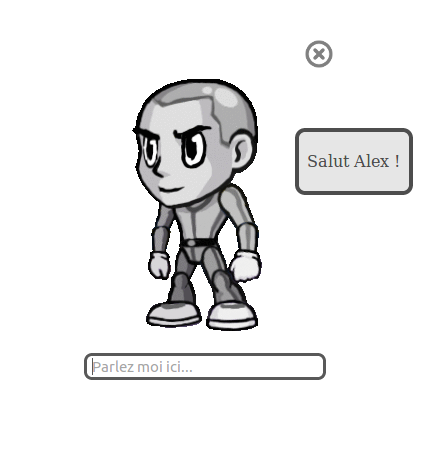
\includegraphics[]{images/agent.png}
 
\endgroup
\vspace*{\fill}


\newpage
\tableofcontents

\newpage


\chapter{Introduction}
	Ce projet, tutoré par Alexandre Pauchet, enseignant chercheur à l'INSA Rouen Normandie est réalisé dans le cadre de la formation ASI de l'INSA Rouen en tant que PAO.\\ 
	
	Il s'agit d'un plugin JQuery dont le but est d'apporter aux développeurs d'applications Web des outils pour assister les utilisateurs de leurs produits à l'aide d'un agent capable d’interagir avec les utilisateurs.\\
	
	Ce PAO avait déjà fait l'objet d'un travail en 2013 par Alexandre Guignebert et Lucie Le Borgne, ainsi qu'en 2014 par Cédric Cousseran et Nicolas Monet.\\
	
	Ce document constitue le rapport du travail effectué sur ce plugin durant l'année 2016-2017.
	
	\section{Méthodologie}
	
	Ce PAO suit une méthode de travail très en vogue ces derniers temps : la méthode agile. Contrairement au cycle en V, elle consiste à travailler sur des tâches plus courtes sur des petites périodes, 1 semaine dans notre cas. C'est ainsi que chaque semaine une réunion a lieu avec le tuteur Mr Alexandre Pauchet pour faire un bilan du travail effectué et décider de la tâche à effectuer pour la semaine suivante.
	
	\section{Spécifications}
	
	Les navigateurs ciblés par le plugin restent les mêmes que les années précédentes, à savoir principalement Chrome, Firefox et Safari.\\
	
	Voici les fonctionnalités que le plugin doit respecter : \\
	\begin{itemize}
	\item L'utilisateur doit pouvoir écrire un message à l'agent via une entrée clavier
	\item L'utilisateur doit pouvoir fermer l'agent s'il le désire
	\item L'utilisateur doit pouvoir déplacer l'agent
	\item L'agent doit être en mesure de répondre à la question de l'utilisateur
	\item L'agent doit être doté d'animations
	\item L'agent doit être interactif
	\item Le développeur qui sera utilisateur de notre plugin doit pouvoir le configurer et créer ses propres fonctionnalités \\
	
	\end{itemize}
	
\chapter{L'existant}

	Ce PAO ayant déjà fait l'objet d'un travail les années précédentes, voici l'état actuel du plugin avant cette session 2017 :
	
	\section{L'agent web}
	
	L'interface de l'agent est déjà présente et peut être déplacée par l'utilisateur grâce à la fonction "drag'n drop".
	
	 \section{Dialogue avec l'utilisateur}
	 
	 Au début du PAO, l'agent était en mesure de répondre à quelques questions de l'utilisateur via une entrée input en html. Si la question n'est pas reconnue, l'agent répond qu'il n'a pas compris la question. La réponse de l'agent est matérialisé sous forme d'une bulle. La librairie TTS (TEXT TO SPEECH) utilisée est celle de Mespeak, située localement. Le système de dialogue est fait de manière "naïve" : chaque question/réponse est stockée dans un fichier xml.
	 
	 \section{Animations}
	 
	 L'agent possède quelques images qui s'affichent en fonction de l’interaction avec l'utilisateur : si ce dernier clique sur l'agent, l'image change, et il en va de même s'il double-clique : l'image de l'agent disparaît alors.
	 
	 \section{Personnalisation du plugin par les développeurs}
	 
	 Une interface php est présente, dont l'objectif et de permettre aux développeurs de personnaliser l'agent pour l'usage qu'ils veulent en faire pour leurs applications web.
	 
	 \section{Bugs et dysfonctionnements}
	 
	 Au début de ce PAO le plugin possédait de nombreux dysfonctionnements : l'agent qui disparaît, l'entrée clavier pour l'utilisateur qui ne suit pas ou mal l'agent lorsque ce dernier est déplacé, la bulle de réponse qui écrase l'agent lorsque l'on déplace ce dernier, le fond blanc qui empêche de voir le contenu de la page derrière l'agent et la voix de l'agent peu agréable (voix robotisée).\\
	 
	 Concernant les fichiers sources : le script php dont l'objectif est de permettre au développeur de personnaliser le plugin ne fonctionne pas ou très mal, et le script js contenant la logique du plugin est condensée en un seul morceau de 1000 lignes.
	 
\chapter{Objectifs de cette session}

	Comme nous travaillons en méthode agile, nous définissons les tâches à réaliser chaque semaine, cependant une liste d'objectifs potentiels à remplir à été effectuée au début de la reprise de ce PAO :\\
	
	\begin{itemize}
	\item Réécrire le plugin en suivant une logique POO (programmation orientée objet) et en séparant les différents modules (animations, dialogues,...) de façon a rendre le projet beaucoup plus maintenable pour les années à suivre.
	\item Régler les dysfonctionnement cités précédemment.
	\item Développer la partie animation dynamique du plugin.
	\item Complexifier la partie dialogue de l'agent.
	\item Reprendre et développer la personnalisation du plugin.
	\item Reprendre l'outil de personnalisation pour les développeurs.\\
	\end{itemize}
	
	A l'écriture de ce rapport, l'ensemble de ces tâches à été réalisé, à l'exception de la complexification de la partie dialogue et animation de l'agent.
	
\chapter{Travail effectué}

	\section{Réécriture du plugin}
	
	Le plugin a été repris a 90\%. Le script js qui contenait la logique de l'agent (et plus de 1000 lignes de code) a été en grande partie restructurée. Les modules dialogues et animations ont été structurés et le script suit maintenant une programmation orientée objet. Voici la nouvelle structure des fichiers sources du plugin :\\
	
	
	dans \emph{agentWeb/js/} : \\
	
	\begin{itemize}
	\item bootstrap/ : contient les librairies js de bootstrap.
	\item classes/ : contient les classes du plugin.
	\item utils/ : contient les scripts des modules dialogues et animations.
	\item script-agentWeb.js : le script-principal qui connecte tout ce beau monde.\\
	\end{itemize}
	
	\section{Interface de l'agent web}
	
	L'interface de l'agent web à été reprise de zéro. Au début, L'agent web était affiché linéairement avec du rafistolage css entre l'image de l'agent, la bulle et l'entrée textuelle. Maintenant, l'agent web est structuré selon le principe suivant : \\
	
	Le bloc de l'interface (ie l'agent) contient 4 blocs : un bloc pour afficher les animations et le personnage de l'agent web, un bloc qui contient l'entrée textuelle, un bloc qui contient la bulle de réponse, et un bloc qui contient une croix permettant à l'utilisateur de faire disparaître l'agent s'il le souhaite. Chaque élément est une instance (un objet donc) de classes définies dans \emph{agentWeb/js/classes/}.\\
	
	Ces éléments possèdent une position et une taille initiales fixes prédéfinies dans le fichier de style   \emph{agentWeb/css/agentWebStyle.css}. Elles ont été choisies de telle sorte à ce que l'agent se situe à droite de l'écran, évitant ainsi d'écraser le contenu central de la page. Dans une majeure partie des sites web, cette partie à droite est soit vide, soit occupée par une publicité. Ce choix permet donc de minimiser une potentielle gène que l'utilisateur pourrait ressentir à son arrivée sur la page.\\
	
	Lorsque l'utilisateur déplace l'agent, sa position s'adapte automatiquement grâce au script \emph{agentWeb/js/utils/dynamicStyle.js} qui modifie les styles des éléments en fonction de la situation, de telle sorte à toujours offrir à l'utilisateur un design responsive et agréable à utiliser. La taille reste toujours fixe quant à elle.\\
	
	En JavaScript, la notion de super classe est très relative, mais chaque objet est un élément du DOM de la page web. On peut donc les obtenir de 2 façons : soit en manipulant le DOM, soit en manipulant les fonctions prévues à cet effet dans leur classes.\\
	
	Par défaut, l'agent a un comportement "idle", que vous avez pu observer à la page de garde de ce rapport. Ils sont tous instanciés dans le script "main" du plugin , à savoir \emph{agentWeb/js/script-agentWeb.js}. Voici un bout du script : \\
	
	\begin{lstlisting}
   var agentWeb = new Agent("agentWeb",xml);
   var inputText = new Question("div","question",xml);
   var character = new Character("div","agent");
   var bulle = new Bulle("div","answer");
\end{lstlisting} 	
	
	A tout moment, l'utilisateur peut cliquer sur l’icône de suppression en haut a droite de l'agent, ce qui permet de le faire disparaître.
	

	\section{Animations}
	
	Le système d'animations a été repensé : les images statiques ont été remplacées par des images dynamiques (ou gifs). Chaque animation est jouée dans le cadre d'une action prédéfinie par le développeur. En effet, l'agent web est maintenant capable d’interagir avec l'utilisateur à travers un ensemble d'actions.\\
	 
	Une action est définie par plusieurs éléments :\\
	\begin{itemize}
	\item une animation (un gif)
	\item une durée d'animation
	\item un message de l'agent pour l'utilisateur
	\item un event JavaScript (optionnel)
	\item quelques autres paramètres\\
	\end{itemize}
	
	Le plugin possède déjà par défaut quelques actions telles que une réaction de sa part lorsqu'on lui clique dessus, lorsqu'on écrit dans un champ texte ou lorsqu'on le déplace. Par exemple, lorsqu'on lui clique dessus, il joue une animation accompagné par un message pour l'utilisateur. \\	
	
	Le système des actions est défini dans le script \emph{agentWeb/js/utils/actions.js} et sont paramétrées dans le fichier xml suivant : \emph{agentWeb/src/actions.xml}. Pour résumer, chaque action définie et parrametrée dans le fichier xml est implémentée dans le script js. Le développeur peut ajouter ses propres actions en suivant le guide de l'utilisateur fourni avec ce rapport. Le script \emph{actions.js} utilise l'introspection pour pouvoir exécuter toute nouvelle action implémentée par le développeur : \\
	\begin{lstlisting}
function loadAllActions(agentWeb,xml){
  	var actions = xml['actions'].getElementsByTagName("action"); <@\textcolor{gray}{//On récupère l'objet SimpleXMLElement qui contient l'ensemble des nœuds de chaque action définies dans actions.xml.}@>
  	animIdle = (actions[1].getElementsByTagName("anim")[0].childNodes[0].nodeValue);
  	for (i = 1; i < actions.length; i++){
  	<@\textcolor{gray}{//On prépare chaque action parramétrée dans le xml et implémentée dans le script js en les appelant comme suit :}@>
    	if ((actions[i].getElementsByTagName("on")[0].childNodes[0].nodeValue) === "true")
     	window[actions[i].getElementsByTagName("name")[0].childNodes[0].nodeValue](agentWeb,xml,actions[i]);
     }
}
\end{lstlisting} 

	Comme vous pouvez le remarquer, l'introspection oblige le développeur qui développe son action dans le fichier \emph{agentWeb/js/utils/actions.js} en utilisant l'api à bien la nommer exactement comme il l'a fait dans le xml.\\	
	
	Le plugin propose quelques fonctions au travers d'une API que le développeur pourra utiliser pour implémenter ses propres actions de la manière la plus simple possible.\\
	
	Les actions incluses de base suivent scrupuleusement ce schéma : elles ont été d'abord paramétrées dans le fichier xml, comme décrit ci-dessus, puis implémentées dans le script js en utilisant l'api.
	
	\section{Dialogue}
	
	Le système de dialogue n'a pas beaucoup changé. Au moment où ce rapport est rédigé, les dialogues se font toujours de manière "naïve" via un xml qui contient les questions et les réponses. Cependant, quelques nouveautés ont été implémentées : les dialogues sont maintenant disponibles en français et en anglais, selon la configuration que le développeur a choisi.\\
	
	 De plus, le vieux moteur TTS meSpeak a été changé par le moteur TTS ResponsiveVoice disponible en ligne et développé en JavaScript par LearnBrite. Il existe plusieurs moteurs TTS en ligne écrits en JavaScript tels que Talkify\footnote{http://talkify.net/text-to-speech-javascript-api}, speechSynthesis\footnote{https://www.npmjs.com/package/tts-js}, et d'autres proposés sur GitHub par des développeurs indépendants. Mais c'est finalement ResponsiveVoice qui à été retenu car c'est celui le plus largement utilisé, la voix obtenue est beaucoup plus agréable audditivement et la librairie est extrêmement facile à utiliser et intégrer à notre plugin.\\
	 
	 Seules 2 lignes de codes suffisent :\\
	\begin{lstlisting}
<script src='https://code.responsivevoice.org/responsivevoice.js'></script>
responsiveVoice.speak("Salut Alex !")
\end{lstlisting}
	
	Le seul désavantage de ce système réside dans le fait qu'elle n'est disponible qu'en ligne, la parole de l'agent web ne sera donc pas disponible hors-ligne, mais ce cas d'usage est extrêmement improbable (On est sur du web là !).
	
	\section{Interface de personnalisation pour le développeur}
	
	L'interface php \emph{agentWeb/configuration.php} pour la personnalisation du plugin par le développeur a été entièrement repensée. Cet outil permet au développeur de modifier directement ses fonctionnalités au travers d'une interface graphique. Voici un aperçu de l'interface :\\
	
	\begin{figure}[H]
\centerline{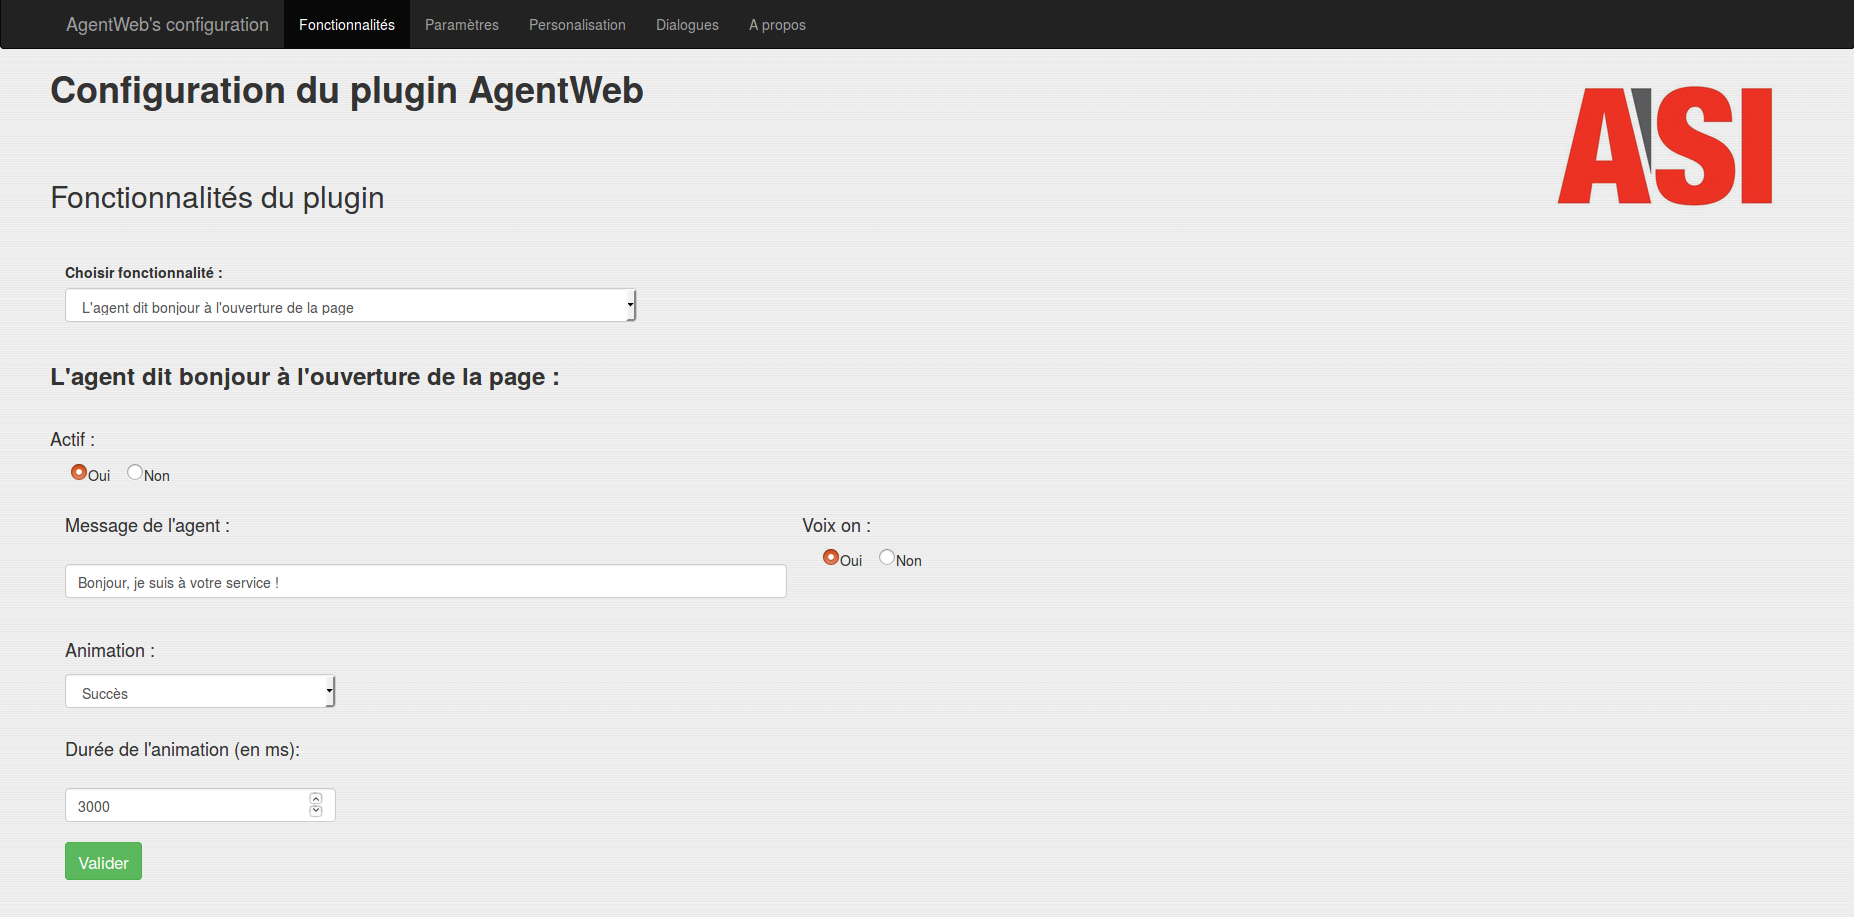
\includegraphics[width=1\textwidth]{images/conf.png}}
\caption{L'interface de personnalisation du plugin}
\end{figure} 
	
	Ce script modifie directement les fichiers de configuration xml situés dans \emph{agentWeb/src} qui servent de paramétrage pour l'agent web, en manipulant leur DOM.
	
	\chapter{Documents de conception}
	
	\section{Diagramme de séquence système}
	\begin{figure}[H]
\centerline{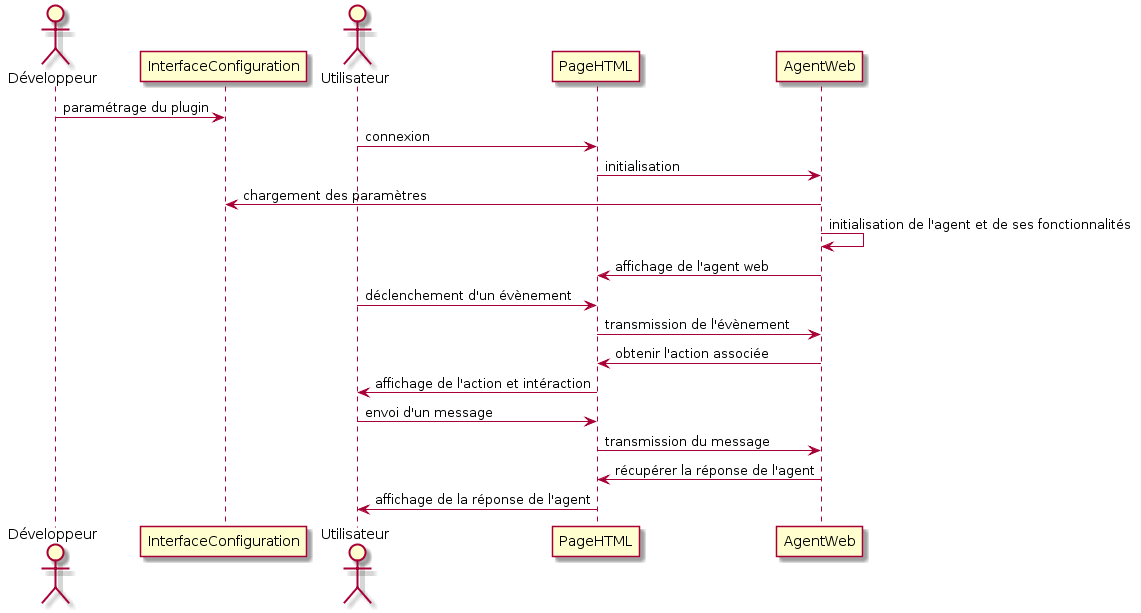
\includegraphics[width=1.2\textwidth]{images/seq_diagram.png}}
\caption{Diagramme de séquence système}
\end{figure}	
	
	\section{Diagramme de classes}
	L'architecture de la logique métier a complètement changée par rapport à la dernière version : en plus des différentes classes, le plugin possède un script helper.js destiné à différentes fonctions comme la recherche dans un XML, et l'initialisation du plugin.\\
	\begin{figure}[H]
\centerline{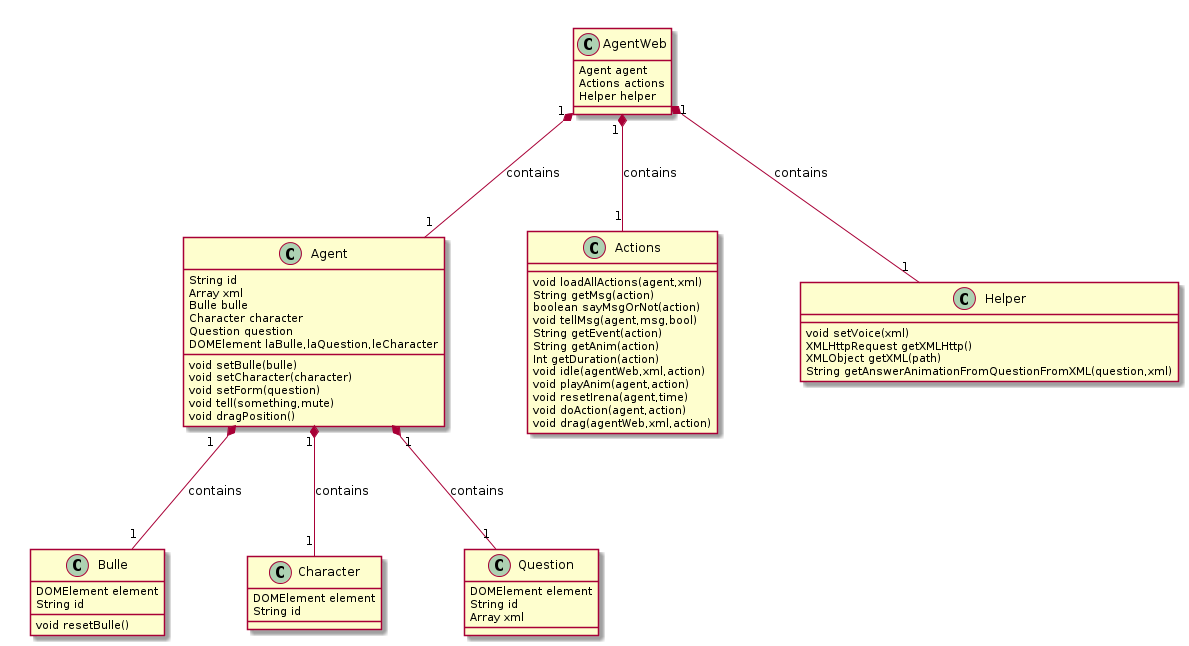
\includegraphics[width=1.2\textwidth]{images/class_diagram.png}}
\caption{Le diagramme de classes du plugin}
\end{figure} 

	\chapter{Améliorations possibles}
	
	\section{Animations}
	Bien que repensé, le système d'animations reste largement perfectible : même si les animations sont maintenant (virtuellement) dynamiques, le développeur reste assez limité : il ne pourra pas faire des animations complexes en choisissant lui même les parties du personnages qu'il veut animer en fonction de la situation. Cette partie étant assez délicate et très complexe, elle pourrait faire l'objet d'un PAO en entier à elle seule.\\
	
	De plus, en dépit de l'introspection utilisée dans les script gérant les actions et de l'API, le développeur doit toujours un peu "mettre les mains dans le cambouis" pour rajouter ses propres animations. En plus de définir les paramètres de sa nouvelle action dans le fichier xml \emph{agentWeb/src/actions.xml}, il doit également implémenter son action dans le script-js prévu à cet effet. Cette implémentation est très simple s'il utilise l'API fournit, mais elle pourrait être évitée avec un système plus poussé. \\
	
	L'interface php de configuration pourrait également être améliorer car elle reste assez dépendante des structures de données déclarées dans les xml.
	
	
	\section{Dialogue}
	
	Le système de dialogue "naïf" peut être amélioré, notamment à travers l'utilisation de ressources indépendantes, telles qu'AgentSlang, qui offre un système de reconnaissance relativement poussés des phrases de l'utilisateur, principalement en s'appuyant sur l'utilisation de synonymes (ex : Syn!bad).
	
	\chapter{Bilan}
	
	Au cours de ce PAO, le plugin a connu de très gros changements : restructuration du code, POO, restructuration du système d'animations, restructuration du système de configuration de l'agent par le développeur (utilisateur de notre plugin),.... L'agent web s'est vu doté de nouvelles fonctionnalités telles qu'une voix plus belle, une interface mieux pensée et structurée, un système d'actions dynamique, ainsi qu'une meilleure gestion de la personnalisation pour le développeur. \\
	
	Le principal objectif de ce PAO a été de rendre le plugin beaucoup plus maintenable et moderne, et de "revenir" à sa fonction primaire, à savoir fournir aux développeurs un outil configurable pouvant interagir avec les utilisateurs de l'application web. \\
	
	Le plugin est maintenant configuré de telle sorte à ce que les futurs développeurs de ce dernier puissent ce concentrer sur les fonctions d'animations et de dialogues, qui, avec beaucoup de recherche et d'investissement, peuvent offrir une très grande capacité d'interaction avec les utilisateurs.\\
	
	La méthode agile à été très bien adaptée à ce PAO : elle a permis de bien mieux évaluer et estimer les différentes tâches, pour ainsi se concentrer sur les plus intéressantes pour le plugin.\\
	
	Personnellement, ce PAO m'a énormément apporté sur le plan technique et conceptuel : j'ai manipulé plusieurs langages de façon très approfondie (php, JS, xml,...) mais en gardant toujours un recul sur le travail à faire en me posant toujours cette question, qui me sauve souvent la mise : "Quel est mon problème ? Quelles solutions ? Quelle solution est la meilleure ?".
\end{document}